%!TEX TS-program = xelatex                                              % 使用xelatex进行处理
%!TEX encoding = UTF-8 Unicode                                          % 使用UTF-8, Unicode

\documentclass[12pt, a4paper]{ctexart}

%%%%%%%%%%%%%%%%%%% 使用包 %%%%%%%%%%%%%%%%%%%

\usepackage{float}
\usepackage{titlesec,shorttoc}
\usepackage{indentfirst}                                                % 首行缩进
\usepackage[colorlinks=true]{hyperref}
\usepackage{fontspec,xunicode,xltxtra}
\usepackage[top=1in,bottom=1in,left=1.25in,right=1.25in]{geometry}
\usepackage{graphicx}
\usepackage{enumitem}
\usepackage{color}
\usepackage{xcolor}
\usepackage{multirow}
\usepackage{url}
\usepackage{bm}
\usepackage[most]{tcolorbox}
\usepackage{fancyhdr}
\usepackage{changepage}
\usepackage{natbib}
\setcounter{secnumdepth}{2}
\setcounter{tocdepth}{2}

%%%%%%%%%%%%%%%%%%% 设置字体 %%%%%%%%%%%%%%%%%%%

\defaultfontfeatures{Mapping=tex-text}
\setmainfont{STKaiti}
\setsansfont[Scale=MatchLowercase]{Gill Sans}
\setmonofont[Scale=MatchLowercase]{Menlo}
\setCJKmainfont{STKaiti}

%%%%%%%%%%%%%%%%%%% 样式设置 %%%%%%%%%%%%%%%%%%%

\hypersetup{urlcolor=Gray, citecolor=Gray}                              % 设置超链接和引用的颜色

\setlength{\parindent}{2em}                                             % 首行空两字
\addtolength{\parskip}{.4em}

%%%%%%%%%%%%%%%%%%% 开始文档 %%%%%%%%%%%%%%%%%%%

\begin{document}

\title{JustRecipes}
\author{\bfseries 笈川伊織\footnote{https://github.com/IoriOikawa/JustRecipes}}
\date{}

\maketitle
\setcounter{secnumdepth}{2}
\tableofcontents

%%%%%%%%%%%%%%%%%%% Beverage %%%%%%%%%%%%%%%%%%%
\newpage
\section{Beverage}

%%%%%%%%%%%%%%%%%%% Beverage - 懒人冷萃咖啡 %%%%%%%%%%%%%%%%%%%
\subsection{懒人冷萃咖啡}
\subsubsection{准备}
\begin{itemize}
    \item{一个干净的容器w}
    \item{冰箱w}
    \item{咖啡粉w}
    \item{法压壶w}
\end{itemize}

\subsubsection{步骤}
\begin{enumerate}[start=0]
    \item{将3份咖啡粉倒入容器}
    \item{向容器中加7份水}
    \item{再在容器中加3份咖啡}
    \item{不许摇晃容器,放入冰箱,温度调至0~4度}
    \item{24~48小时后拿出容器,过法压壶}
    \item{0~4度且未加糖时,容器可以保存两星期}
\end{enumerate}

\subsubsection{PS}
推荐配糖浆及冰块饮用 不喜欢咖啡的酸味的话超级推荐

\subsubsection{PPS}
注意饮用量,当心手抖w

%%%%%%%%%%%%%%%%%%% Beverage - 三秒葡萄酒 %%%%%%%%%%%%%%%%%%%
\subsection{三秒葡萄酒}
\subsubsection{准备}
\begin{itemize}
    \item{标有 \textbf{Nectar} 字样,或者高甜度的葡萄汁w}
    \item{威士忌w}
    \item{纸和笔w}
    \item{当然还有脑子w}
\end{itemize}

\subsubsection{步骤}
\begin{enumerate}[start=0]
    \item{拿出葡萄汁,注意一定要选择甜的}
    \item{选择好的威士忌}
    \item{拿出纸笔}
    \item{高中化学浓度计算,控制酒精度至 3\%~5\%}
    \item{或者如果想让今天过去的话,控制酒精浓度在 9\%~13\%}
    \item{或者你丫不喜欢葡萄味儿,那就直接喝吧。。。}
    \item{高于 13\%,市面上只有浓缩葡萄汁才可能中和酒精气味}
\end{enumerate}

\subsubsection{PS}
可以把配好的葡萄汁放入冰箱,此时不用担心分层
或者莓果类甜型果汁也可,但选用果汁必须澄清

\subsubsection{PPS}
根据某傻喵统计,此剂酒精含量与醉倒人数呈现正态分布

%%%%%%%%%%%%%%%%%%% Beverage - 三周葡萄酒 %%%%%%%%%%%%%%%%%%%
\subsection{三周葡萄酒}
\subsubsection{准备}
\begin{itemize}
    \item{标有 \textbf{Nectar} 字样,或者高甜度的葡萄汁w}
    \item{两大勺糖(按 1L 果汁计)}
    \item{气球}
    \item{针}
    \item{好用的日历}
\end{itemize}

\subsubsection{步骤}
\begin{enumerate}[start=0]
    \item{拿出葡萄汁,注意一定要选择纯的}
    \item{每升果汁加入 60~150g 的糖}
    \item{60~90g = 干型葡萄酒 >90g = 甜型}
    \item{拿气球套在饮料瓶口,用针戳 4~6 个小孔}
    \item{孔的位置必须在瓶口被气球绷紧的位置}
    \item{或者你丫喜欢葡萄味醋,那就自便吧。。。}
    \item{将整个劳什子放到冷暗处,温度控制在 18 度~ 24 度}
    \item{等两至三周即可}
\end{enumerate}

\subsubsection{PS}
或者莓果类甜型果汁也可,最好再加入 10\% 质量的碾碎水果
至于时间。。。自己拿捏吧。。。等做完实验再说w

\subsubsection{PPS}
如果更想体会 3 年葡萄酒,把葡萄汁换成葡萄就好
注意密封,温度控制在 16~18 度
加一句,葡萄皮必须留一部分带白霜的
那个不是白霜,是酵母菌哟

%%%%%%%%%%%%%%%%%%% Domintory Recipes %%%%%%%%%%%%%%%%%%%
\newpage
\section{Domintory Recipes}

%%%%%%%%%%%%%%%%%%% Domintory Recipes - 宿舍用火锅 %%%%%%%%%%%%%%%%%%%
\subsection{宿舍用火锅}
\subsubsection{准备}
\begin{itemize}
    \item{一个保温杯w}
    \item{一个水壶w}
\end{itemize}

\subsubsection{步骤}
\begin{enumerate}[start=0]
    \item{底料放水壶里热一下拿出来,算是第一锅}
    \item{蓝后第二锅用水壶}
    \item{加水放次的}
    \item{涮之}
    \item{涮好的放保温杯蘸底料}
\end{enumerate}

\subsubsection{PS}
害怕辣或者想蘸底料就单独拿一个一次性杯子或者碗放底料就好

\subsubsection{PPS}
虽然大块的东西像是脑花不一定能入味儿倒是

%%%%%%%%%%%%%%%%%%% Domintory Recipes - 最完美的溏心蛋 %%%%%%%%%%%%%%%%%%%
\subsection{最完美的溏心蛋}
开水壶溏心蛋
\subsubsection{准备}
\begin{itemize}
    \item{一个鸡蛋w}
    \item{一个水壶w}
    \item{计时工具w}
\end{itemize}

\subsubsection{步骤}
\begin{enumerate}[start=0]
    \item{将水加热,可以加入盐/胡椒}
    \item{等水沸腾后快速搅动水呈漩涡状}
    \item{趁漩涡在时将鸡蛋一整个打到水里}
    \item{计时90~120秒,蛋一定是溏心的}
    \item{拿个勺子捞出来就可以了}
\end{enumerate}

\subsubsection{PS}
想在宿舍里吃方便面加溏心蛋的话,就把盐/胡椒换成方便面底料,然后做溏心蛋。将蛋捞出再加面饼煮就可以了w

\subsubsection{PPS}
漩涡的水流将会让蛋白保持在蛋黄周围。哪怕是最高级的酒店,做溏心蛋用的也是这个方法哦,虽然不是用热水壶,而是锅子就是。

%%%%%%%%%%%%%%%%%%% 毒品改造计划 %%%%%%%%%%%%%%%%%%%
\newpage
\section{毒品改造计划}

%%%%%%%%%%%%%%%%%%% 毒品改造计划 - 戴白花的血腥玛丽 %%%%%%%%%%%%%%%%%%%
\subsection{戴白花的血腥玛丽}
白花蛇草水改造计划1 - 无酒精血腥玛丽+

\subsubsection{准备}
\begin{itemize}
    \item{白花蛇草水 60 毫升w}
    \item{一个冰箱w}
    \item{冰块w}
    \item{一截又粗又大的芹菜杆w}
    \item{番茄汁 150 毫升w}
    \item{一点香菜w}
    \item{半个柠檬w}
    \item{合适的杯子w}
    \item{马桶w}
\end{itemize}

\subsubsection{步骤}
\begin{enumerate}[start=0]
    \item{把冰箱门打开}
    \item{把白花蛇草水装进冷藏室}
    \item{把柠檬扔进冷冻室}
    \item{把冰箱门关上}
    \item{啊关之前别忘了做冰块~}
    \item{把冰箱门打开}
    \item{把冷藏的白花蛇草水和冻好的冰块拿出来}
    \item{将番茄汁、白花蛇草水混合}
    \item{解冻后榨干可怜的半个柠檬}
    \item{冰箱门要常关~}
    \item{把柠檬汁加进白花番茄汁里}
    \item{把成品倒入杯子,加冰}
    \item{那截又粗又大的芹菜杆就拿来当吸管吧}
\end{enumerate}

\subsubsection{改造要点}
白花蛇草水本身保健效果拔群,非常适合扁桃体炎的缓解和治疗,咽炎和因雾霾导致的不适感也都可以缓解,其药用价值难得地被医学界证明过。

白花蛇草水的死穴是饮用的温度,如果太高,草的味道就会破坏感觉,在0~10度时,那种味道则会收敛,变成一种近似于胡椒皮的风味,所以它可以作为无酒精血腥玛丽配方里,胡椒、辣椒粉温柔的替代品。

\subsubsection{PS}
如果喜欢这种若隐若现的味觉,天生排斥带有胡椒辣椒的鸡尾酒的话,也可以在此配方的基础上,加入30毫升的伏特加,同时将白花蛇草水用量减半,便会得到比较温柔的血腥玛丽了。

%%%%%%%%%%%%%%%%%%% 毒品改造计划 - 停不下来的火鸡年糕 %%%%%%%%%%%%%%%%%%%
\subsection{停不下来的火鸡年糕}
火鸡面改造计划 芝士年糕火鸡面(2 - 3人份)

\begin{figure}[!t]
    \centering
    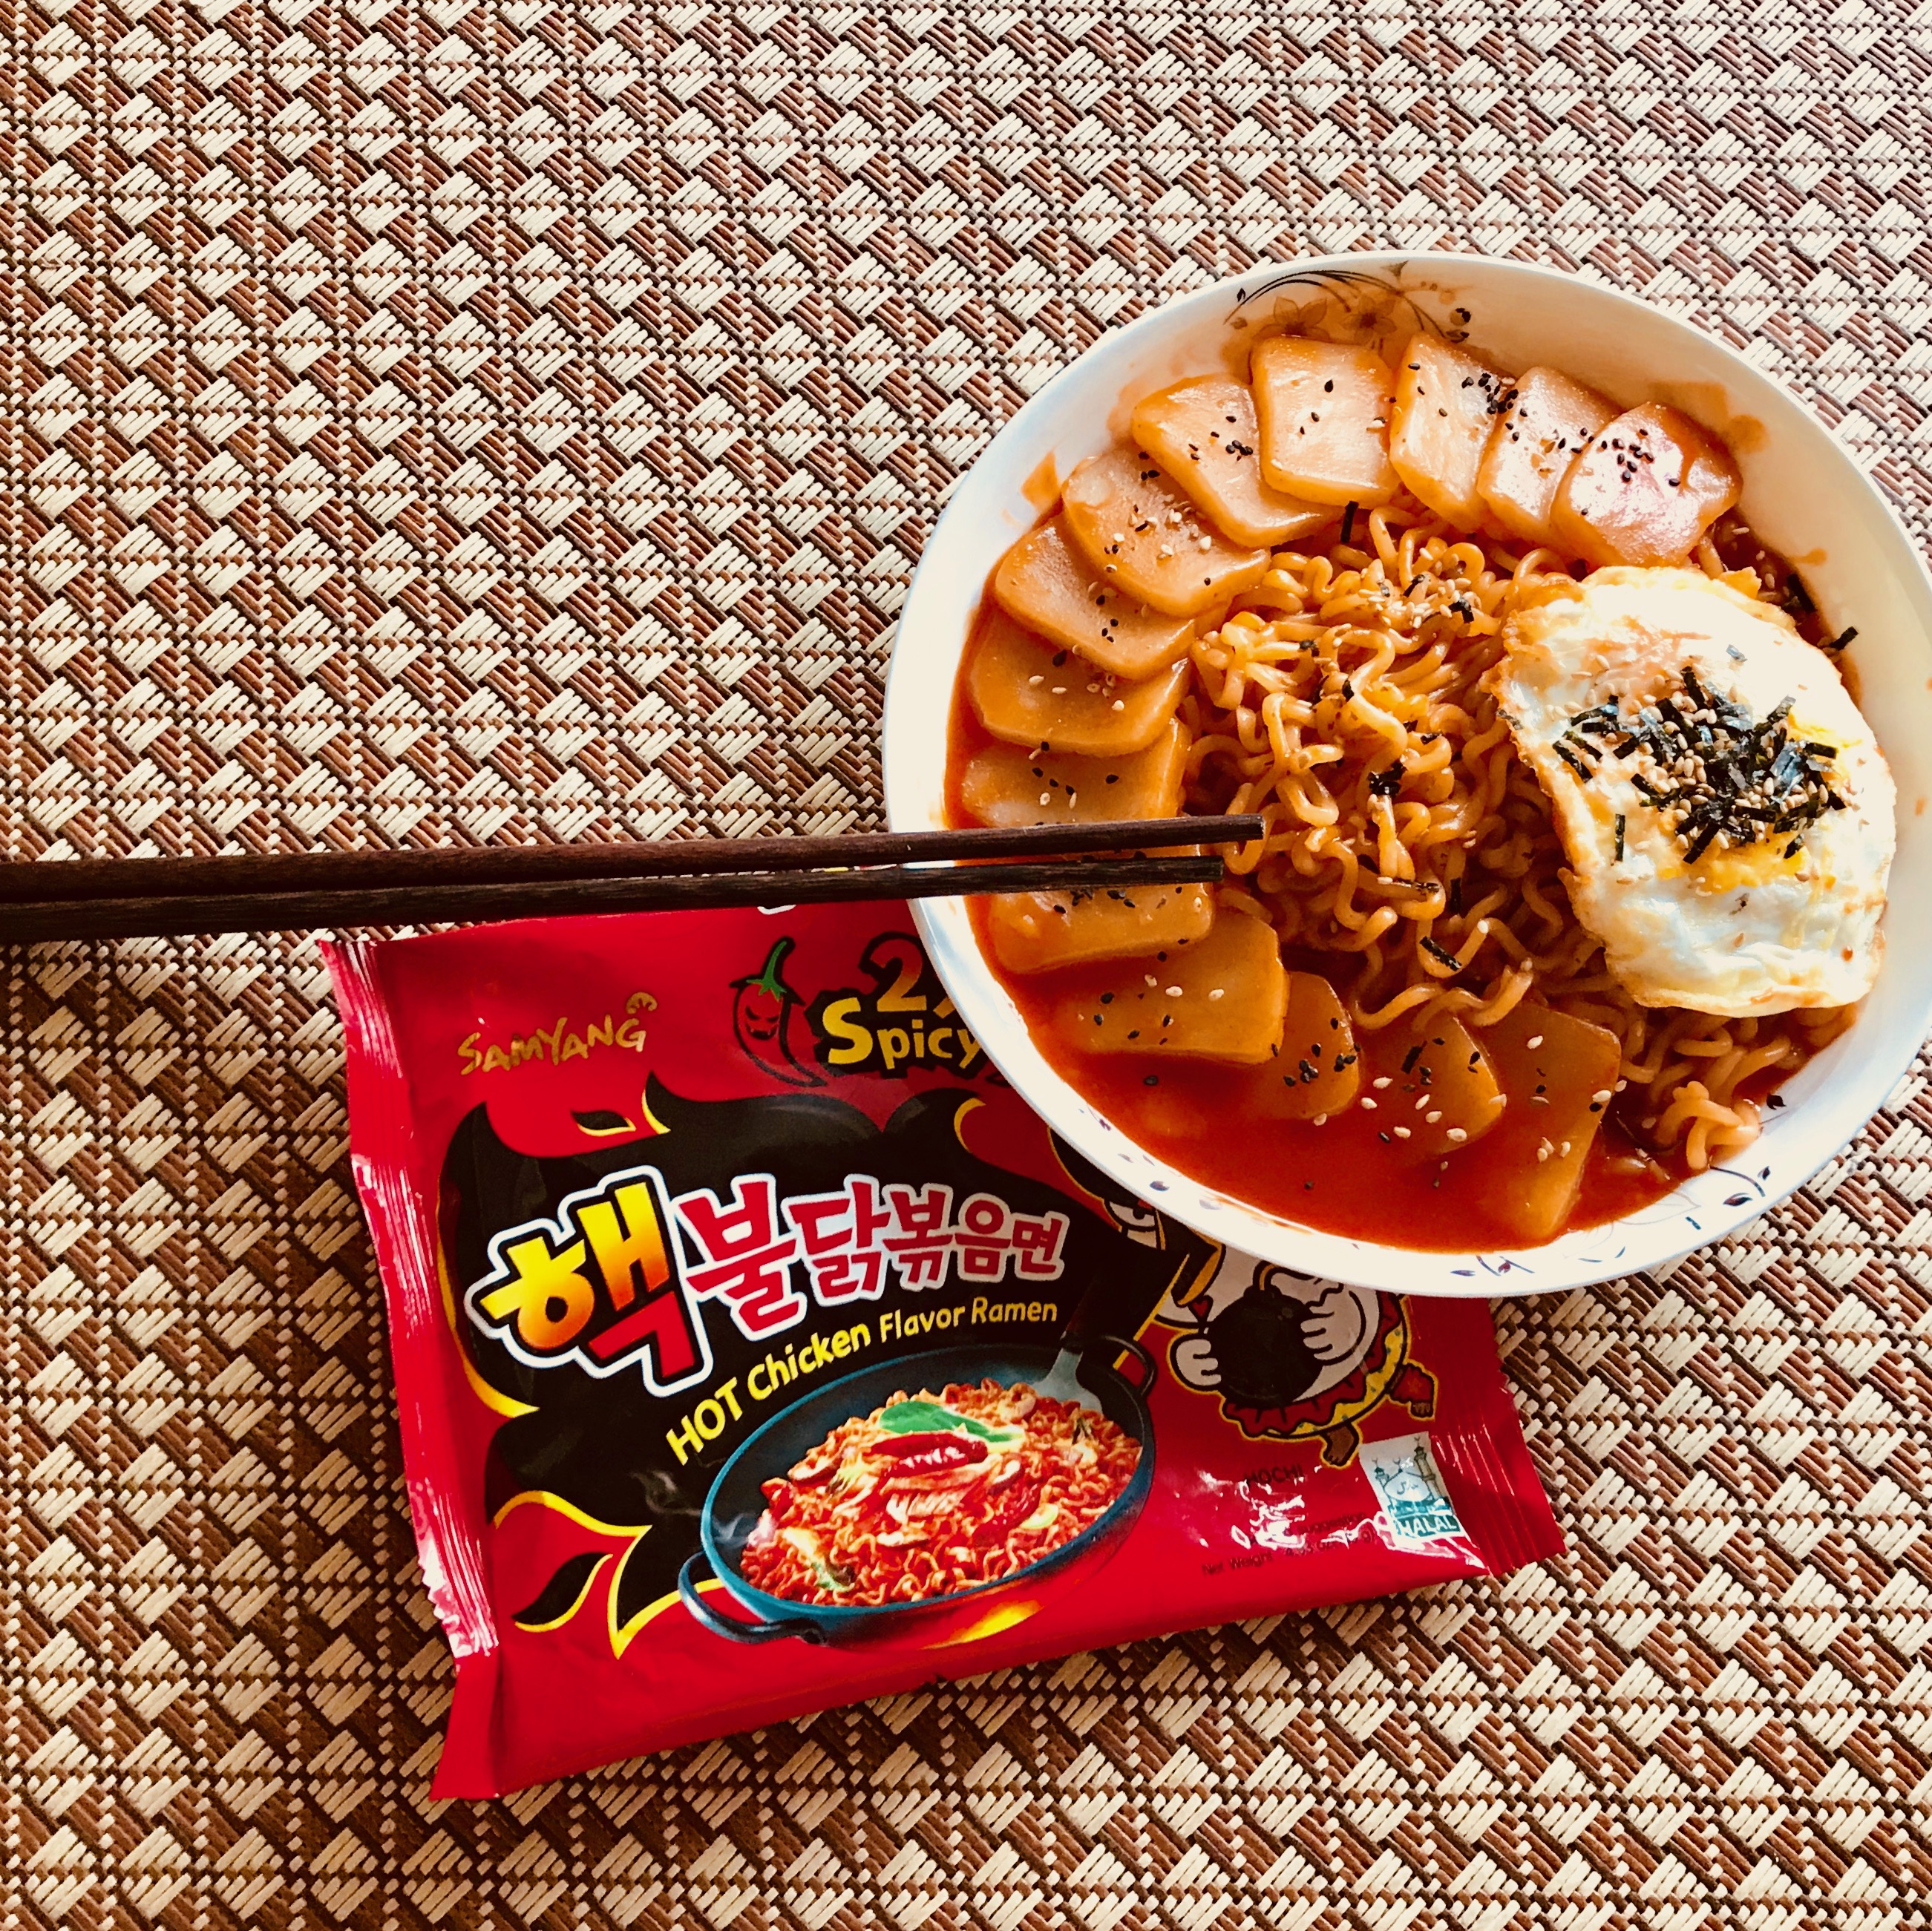
\includegraphics[width=3.2in]{figures/hot-chinken-ramen-with-mochi-figure-1}
    \caption{停不下来的火鸡年糕-1}
    \label{hot-chinken-ramen-with-mochi-figure-1}
\end{figure}

\begin{figure}[!t]
    \centering
    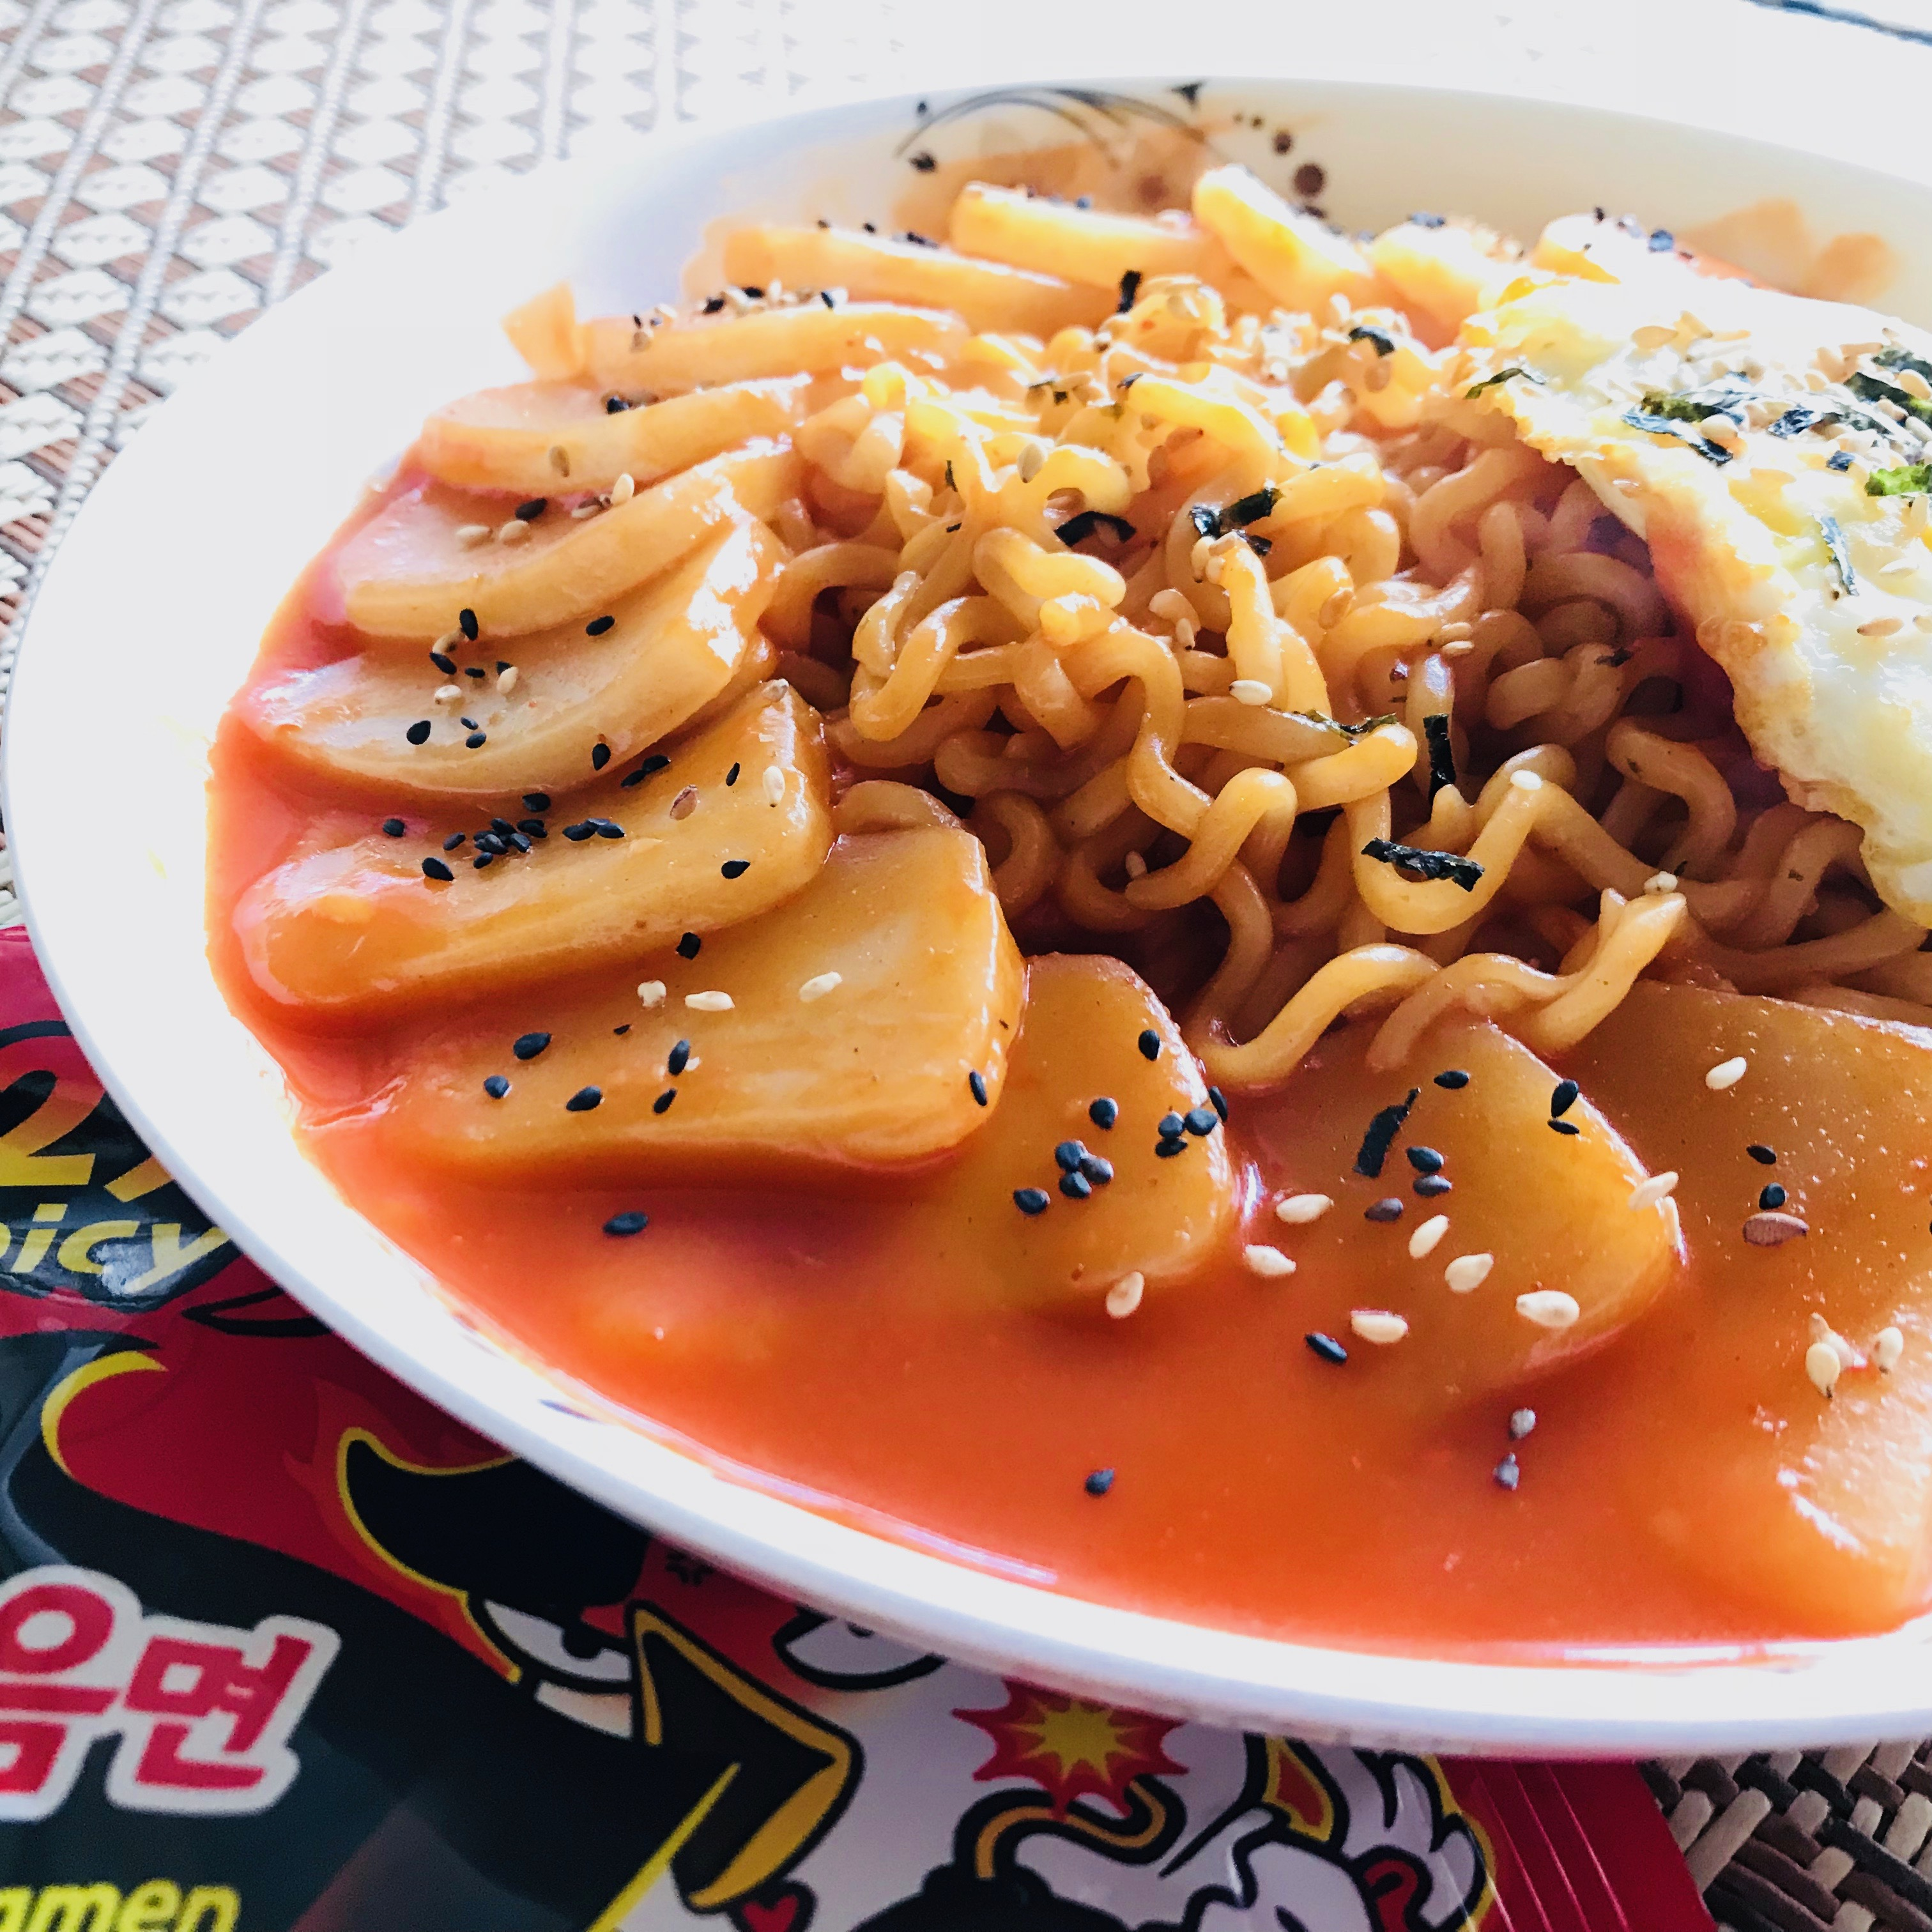
\includegraphics[width=3.2in]{figures/hot-chinken-ramen-with-mochi-figure-2}
    \caption{停不下来的火鸡年糕-2}
    \label{hot-chinken-ramen-with-mochi-figure-2}
\end{figure}

\subsubsection{准备}
\begin{itemize}
    \item{火鸡面一包w}
    \item{奶酪丝 50 克w}
    \item{火锅年糕 150 克w}
    \item{卡夫芝士粉w}
    \item{芝麻及海苔碎w}
    \item{亨氏番茄酱 50 克w}
    \item{一个锅子w}
    \item{一位重庆/四川/湖南/江西人w}
\end{itemize}

\subsubsection{步骤}
\begin{enumerate}[start=0]
    \item{开水煮面和年糕}
    \item{煮好后将水倒掉剩下 100 毫升+}
    \item{加入原来的酱料、番茄酱、奶酪丝}
    \item{翻炒 30 秒}
    \item{出锅后撒上芝麻海苔碎,当然也包括料包里的}
    \item{吃 露出笑容 然后再吃 吃到辣哭为止w}
    \item{吃不下去的话,就轮到准备表上的最后一项出场了}
\end{enumerate}

\subsubsection{改造要点}
火鸡面的缺点,是辣的没有内涵。

如果味觉层次丰富一些,也就不会沦为开玩笑的工具啦。

\subsubsection{PS}
如果觉得不够辣,可以将番茄酱换为泰式辣椒酱,一定会让乃欲罢不能www 可是好吃也要量力而行哦。

\end{document}
